\section{Introduction}~\label{intro}

Recent advances in robotic systems have significantly improved autonomy in perception, manipulation, and planning across domains such as agriculture and household environments. Despite these advances, robots still encounter perception errors~\cite{kaipa2016addressing}, action execution failures~\cite{kaelbling1998planning}, and unexpected environmental changes~\cite{kurniawati2016online}. As a result, many robotic systems continue to rely on human operators to monitor execution and intervene when failures occur~\cite{dragan2013legibility, goodrich2008human}. However, requiring humans to continuously monitor robotic systems and determine whether robot decisions are correct is impractical in long-horizon tasks because it increases cognitive workload and fatigue~\cite{chen2014human}. Instead of relying on human operators to detect failures after they occur, robotic systems should be able to recognize uncertain situations during execution and request assistance only when additional information is required~\cite{sadigh2017active, leusmann2023understanding}. This raises two fundamental questions: (i) when should a robot request human assistance, and (ii) what information should it request?


Recent studies have explored uncertainty-aware robotic systems that selectively request human feedback during task execution~\cite{ren2023robots, liang2024introspective, mullen2025lbap}. These approaches demonstrate that uncertainty-aware querying can reduce unnecessary human intervention and improve decision making under uncertainty.However, uncertainty estimation, query generation, and planning are often treated as separate components. As a result, the relationship between when to request human assistance, what information to request, and how the acquired feedback should influence subsequent decision making remains insufficiently explored in robotic systems operating under uncertainty.

To address this challenge, we propose a knowledge-based robotic framework that integrates uncertainty estimation, query selection, and task planning into a unified decision-making process.
% To address this challenge, we propose a knowledge-based robotic framework that selectively incorporates human feedback during task execution. 
We formulate decision making as a partially observable Markov decision process (POMDP)~\cite{kaelbling1998planning} and represent task knowledge using a STRIPS-style symbolic model~\cite{davis1993knowledge,fikes1971strips}. The system maintains a belief over alternative world hypotheses and continuously updates this belief using observations collected during execution. The resulting belief distribution is used to determine whether additional information is required. When uncertainty exceeds a threshold, the robot requests feedback that is expected to maximally reduce ambiguity among competing hypotheses. Otherwise, the robot continues autonomous planning and execution.



\begin{figure}[t]
\captionsetup{skip=0pt}
\centering
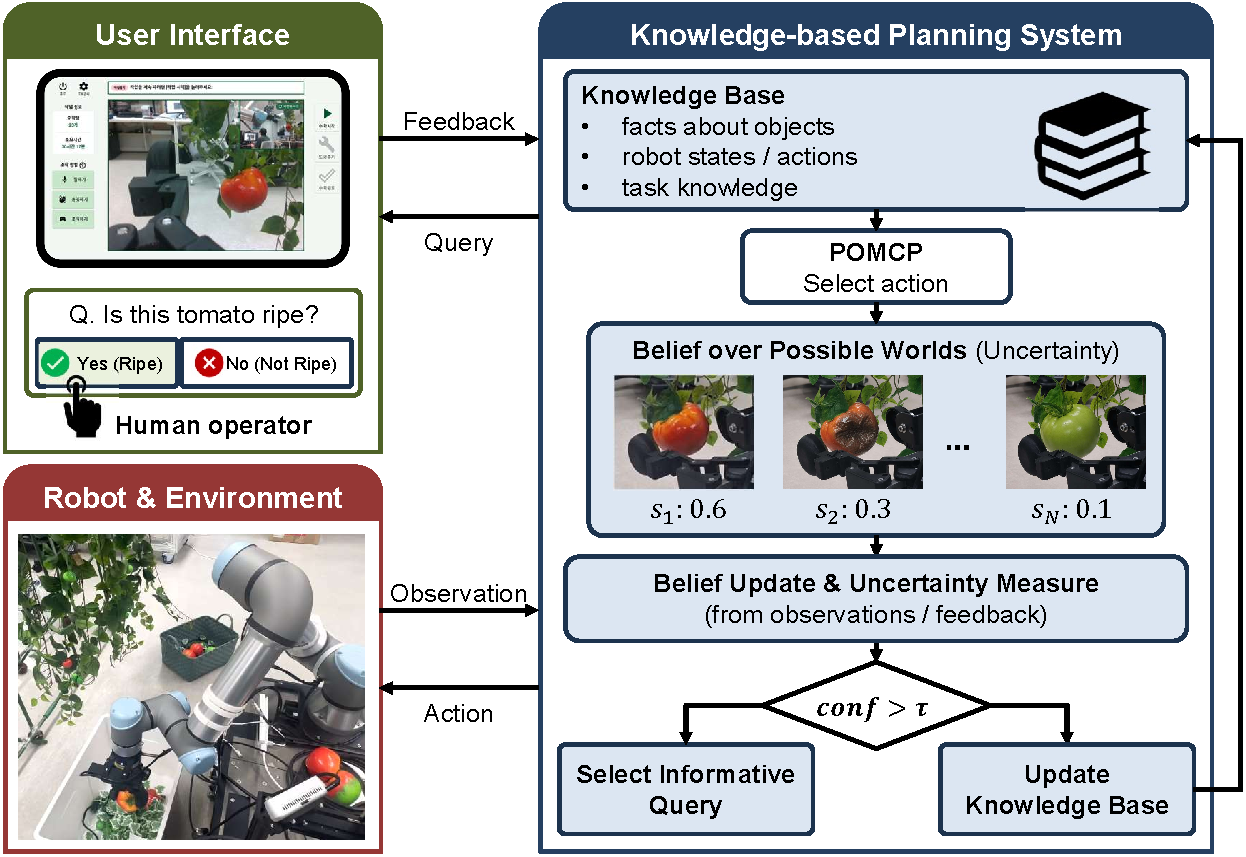
\includegraphics[width=0.7\linewidth]{figures/fig_overview.pdf}
\caption{Overview of the proposed knowledge-based robotic system with uncertainty-aware planning. The system maintains a belief over possible worlds and updates it based on observations. If the uncertainty exceeds a threshold, the system selectively queries the user to resolve ambiguity. Otherwise, it continues autonomous planning and execution.}
\label{fig:intro}
\end{figure}

To support autonomous operation under uncertainty, we integrate the proposed framework into a robotic system architecture. As illustrated in Fig.~\ref{fig:intro}, a centralized knowledge base connects the sensing, planning, feedback management, and user interface modules. Sensor observations and user feedback are stored in the knowledge base and shared across modules, providing a consistent representation of the environment throughout execution. Planning is performed over symbolic world states, while belief updates maintain uncertainty over alternative hypotheses. Consequently, the robot can continue autonomous execution and request human feedback only when necessary.


We evaluate the proposed approach in two robotic domains, tomato harvesting and waste sorting. Experimental results demonstrate that the framework improves task performance while reducing the amount of human intervention required during execution. We further analyze how different query policies influence situation awareness and perceived workload through user studies.

The main contributions of this work are as follows:

\begin{itemize}

\item We propose an uncertainty-aware feedback triggering method for determining when human assistance is required during task execution.

\item We propose an information-driven query selection method for identifying what information should be requested to reduce uncertainty over competing world hypotheses.

\item We incorporate uncertainty-aware querying into the planning and execution process, enabling autonomous robot operation with selective human feedback.

\item We validate the proposed approach in tomato harvesting and waste sorting tasks through robot experiments and user studies.

\end{itemize}
